\documentclass{jssms}
%建议使用此模版前登陆www.ctex.org/CTeXDownload下载Latex软件.
%此模板需调用宏包jssms.cls, 请确保此宏包与tex文件在同一文件夹下.
%请使用CCT&LaTex编译.


\numberwithin{equation}{section}
% 公式编号会随着Section而变动,如(1.1),(1.2),(2.1)...,如果不便使用,您可以将这个命令删去
%--------------文内自定义命令----------------

%实现了用\caption{}可以Figure1 黑体
\usepackage[font=small,labelsep=quad,labelfont=bf,width=\textwidth,format=hang,indention=0mm]{caption}

\usepackage[font=small,labelsep=quad,labelfont=bf]{caption}

\def\RM{\rm}
\def\It{\it}
\def\hat{\widehat}
\def\tilde{\widetilde}
\def\bar{\overline}
\def\epsilon{\varepsilon}
\def\dd{{\rm d}}
\def\ii{{\rm i}}
\def\ee{{\rm e}}
\def\q{\quad}
\def\dint{\displaystyle\int}
\def\vsp{\vspace{1mm}}
\def\no{\nonumber}
\def\q{\quad} \def\qq{\qquad}
\def\ay{\arraycolsep=1.5pt}
\def\d{\displaystyle}
\def\dfrac{\displaystyle\frac}
\def\la {\langle}              \def\ra {\rangle}
\def\n{\noindent}
\def\*{$\!\!^{^{^{\displaystyle *}}}$}
%**************************************************
\def\jssmszi{\zihao{10}\ziju{0.135}}
\parindent=2\ccwd
\def\rmn#1{\romannumeral #1}
\def\Rmn#1{\expandafter\uppercase\expandafter{\romannumeral #1}}
\def\cases#1{\left\{\,\vcenter{\normalbaselines \openup\jot
    \ialign{$\displaystyle{##}$\hfil&\quad{##}\hfil\crcr#1\crcr}}
    \right.}
%---------------------------------------
%--------------文内自定义命令结束------------

%--------------作者自定义命令----------------



%--------------作者自定义命令结束------------

%*************************************************
%***************************************

%-------------正文开始------------------


%%%%%%%注意:全文标点符号请使用英文输入状态下的格式进行排版


\begin{document}

\thispagestyle{empty}


\Volume{20xx}{x}{x}{x}               % 年、月、卷、期
\PageNum{1}                                  % 起始页码
\PaperID{0583-1431(20xx)0x-0xxx-0x}   % 文章编号
\DocumentCode{A}                              % 文献标识码
\EditorNote{*基金项目.}%如 *国家自然科学基金(10171074)资助课题.  如没有基金项目请删去此行


%%%%%%%%%%%%%%%%%%%%%%%%%%%%%%%%%%%%%%%%%%%%%%%%%%%%%%%%%%%%%%%%%%%%%%%%%%%%
%%%%%  作者从下面开始填写各项内容,本刊的标点符号均使用英文标点,您可以在编译前设置标点形式

\EditorNote{收稿日期: 200x-xx-xx, 收到修改稿日期: 200x-xx-xx.}  % 脚注

\EditorNote{通信作者: 姓名, Email:  .}
%只能添加一位作者为通信作者。注意通信邮箱不建议使用QQ等社交软件邮箱。

\EditorNote{编委:  }% 脚注,作者不必填写。


\TitleMark{作者姓名: 论文标题}% 页眉, 如有多位作者,请写为: 第一作者姓名等: 论文标题

 \BeginTitle

\Title{论文标题\*}

\Author{姓名1$^{1}$\q\q 姓名2$^{2}$\q\q 姓名3$^{3}$}%例如: 张\ 小\ 乙$^{1}$\q\q 李\ \ 甲$^{2}$\q\q 刘\ 小\ 丙$^{3}$
 {(1. 作者单位,\, 城市 邮编;\, 2. 作者单位,\, 城市 邮编;\, 3. 作者单位,\, 城市 邮编)}
 %学校全称及二级单位名称; 例如: (中国科学院数学与系统科学研究院系统科学研究所,\, 北京 100190)



\Abstract{摘要内容}

\Keywords{关键词1, 关键词2, 关键词3, $\cdots$.}%甲, 乙, 丙, 丁.

\MRClass{MR分类号1, MR分类号2,...}%注意:不是中图分类号,需作者自己提供.
\DOI{ }%此处括号内填稿件编号即可



\ETitle{English Article's Titles } %英文标题名称,首字母需大写

\EAuthor{\uppercase{XING} Ming1$^{1}$\q\q \uppercase{XING} Ming2$^{2}$\q \q \uppercase{XING} Ming$^{3}$} % 作者姓名的拼音,姓在前,名在后,
{\small(1. {\it Author's Address,\, City} Postcode;\, 2. {\it
Author's Address,\, City} Postcode;\, 3. {\it Author's Address,\,
City} Postcode)}
% 如 \small({\it Academy of Mathematics and Systems Science, Chinese Academy of Sciences,\, Beijing} 100190) \\

%\EAuthor{\uppercase{XING} Ming\q \q \uppercase{XING} Ming}
%{\small(Author's Address)}

%顺序相邻的几个作者若单位相同,合并在一起排版,可参考网站过刊已发表文章中格式。

\EAbstract{In this paper, we $\cdots$}
注意:英文摘要需将文中研究结果和结论尽量详细阐述,使不懂中文的学者能了解
到文章的研究成果.注意语句使用和语法问题.

\EKeywords{Keyword1, Keyword2, Keyword3, $\cdots$.}%Jia, yi, bing, ding.


\EndTitle



\Section{引\ \ 言}

Bustos和Concha\supercite{ref1}讨论了$\cdots$,
其它结论见文献\cite{ref2,ref3,ref4},


公式示例\supercite{ref2,ref3,ref5,ref6,ref7}
\begin{align}\label{eq:1.1}
a&=b \nonumber\\
&=c\nonumber\\
&=d.
\end{align}
其中由式\eqref{eq:1.1}, % 也可以使用(\ref{eq:1.1})来引用公式编号
我们可以得到\FootNote{1.脚注的命令格式.}
\begin{align*}
a=b.
\end{align*}

{\HT 定义 1.1}\ \   内容

{\HT 引理 1.2}\ \   内容

\indent {\FS 证}\ \   内容

{\KS 注 1.3}\ \   内容



注意文中的标点符号应使用英文半角状态下的格式,例如: , . : ; ? ( )
``''等; 使用的大写希腊字母统一要用斜体标示,例如: ${\it \Phi},{\it
\Lambda},
 {\it \Theta},{\it\Omega},\cdots$; 文章中请使用1), 2), 3),
 $\cdots$或 (i), (ii), (iii), $\cdots$ 或 (h), (i), (g), $\cdots$表示
 分类符号; 公式中的微分符号$d$要正体,例: $\int f(x)\dd x$,
  $\dd y(t)=t^2+1$; 常数$e$字体为正体,例: ${\rm e}$或$\ee$,除此之外,
公式序列要先列举两项,再使用省略号 $\cdots$,
 例: $\{f(x_i),\ i=1,2,\cdots,n\}$, $y_1<y_2<\cdots<y_n$,
$A=A_1+A_2+\cdots+A_m$,  $ \cdots$.

\Section{主要定理及其证明}
\setcounter{section}{2}\setcounter{equation}{0}

{\HT 定理 2.1}\ \   内容

\indent {\FS 证}\ \   内容  \Subsection{2.1\ \ 表格示例}
\begin{center}\tabcolsep 2pt %调节表列距
    \centering{\small 表1\ \ 标题}\\
    \centerline{\small (Table 1\ \ English title)}%%表中文标题下附英文标题翻译,第一个单词首字母大写即可。
\vskip 1mm
{\small
\setlength{\tabcolsep}{5pt}  %调节表列距
\renewcommand{\arraystretch}{1.0}%调节表行距
    \begin{tabular*}{6.5cm}{cccccccc}
        \hline
        &\multirow{2}{*}{$\rho$}   &\multicolumn{2}{c}{AR(1)} &   \multicolumn{2}{c}{MA(1)} &    \\

\cmidrule(r){3-4}\cmidrule(r){5-6}
                 &           & $\theta_{0}$ & $\beta_{0}$ & $\theta_{0}$ & $\beta_{0}$   \\
        \hline
            &0.6   &0.0037    &2.1503    &0.0071    &2.1247   \\
            &0.1   &0.0034    &1.8573    &0.0034    &1.7147   \\
            & 0.0   &0.0031    &1.8490    &0.0030    &1.6400   \\
            & 0.1   &0.0033    &2.0329    &0.0035    &2.1271   \\
      \hline
    \end{tabular*}}
\end{center}
%\begin{table} \end{table}环境也可,但图标位置会浮动.

\Subsection{2.2\ \ 图示例}
\begin{center}
\centerline
  {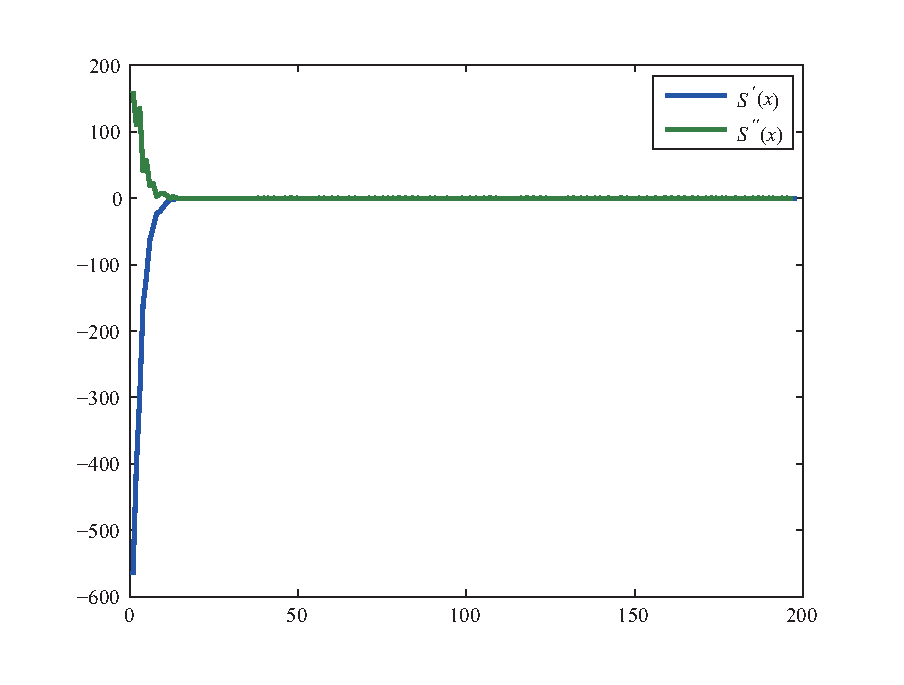
\includegraphics[scale=0.3]{1.eps}}%%需在tex源文件中提供清晰版的eps格式的矢量图文件。
\centering{\small 图1\ \ 标题}\\
 \centerline{\small (Figure 1\ \ English title)}%%图中文标题下附英文标题翻译,第一个单词首字母大写即可。}
\end{center}
其中[scale=0.42]的参数可以调节大小.
%\begin{figure} \end{figure}环境也可,但图位置会浮动.

\addtocounter{subfigure}{-3}

{\KS 注 2.2}\ \
注意文中提供的图要求为清晰的矢量图(eps格式或pdf格式),图为Times New
Roman Regular字体,图中变量符号为Times New Roman
 Italic字体(可使用Adobe Illustrator软件实现),图中所使用的数学符号要与文中格式保持一致.

 \Subsection{2.3\ \ 公式示例}

%----------------------------------
%--文中公式需注意:
%--文中的复杂公式应独立成行,
%--公式格式需规整,
%--公式中括号不应小于其中内容,
%--公式后应有标点符号.
%----------------------------------

\ay
\begin{eqnarray}\label{E:2.1}
AAAAAAAAAA &=& BBBBBBBBBBB\nonumber \\
           && + CCCCCCCCCC\nonumber \\
           &=& DDDDDDDDDDDDD.
\end{eqnarray}
%公式太长时,换行注意相应符号对齐格式.注意,公式长度不能超版芯

\ay
\begin{eqnarray}\label{E:2.2}
&&AAAAAA =(A+B)-\big(B^{-2^A}+1\big)D-C,\nonumber \\
&&BBBBBBBBB=AA-BB+\bigg\{\frac{A}{B}+
\dfrac{B^2-C+\frac{A}{D}}{CC+AD}\bigg\}-CCCC\nonumber \\
&&\hspace{3cm}+DDDDD,\nonumber \\
&&DDDDDDDD={\it \Omega}A+{\it \Phi}_{2}.
\end{eqnarray}
%多行公式时注意左对齐格式;注意实用合适大小的括号.
\ay\begin{align}\label{E:2.3} &A_{1}=B^{\rm T},\q A_{2}=C, \q
A_{3}=D,\\% 注意多个公式之间要用\quad隔开. 矩阵向量的转置符号T要正体.
& AA=\left\{
                   \begin{array}{ll}
                     BBB, \q & C=DD, \\
                     0, \q  & \mbox{其他}.
                   \end{array}
                 \right.
 \end{align}
% 注意各列要左对齐.

%以下为公式排版式例.
\ay
\begin{eqnarray}
\|\tilde{u}^{y}(\cdot,t)\|_{L^{1}}&\leq&
\ee^{\bar{\beta}t}\|u_{0}\|_{L^{1}}
+\d\int_{0}^{t}\ee^{\bar{\beta}(t-s)}\bigg\|
\dfrac{f(\cdot,s)}{y(s)}\bigg\|_{L^{1}}\dd s \nonumber\\
&\leq& \ee^{\bar{\beta}t}\|u_{0}\|_{L^{1}}
+\d\int_{0}^{t}\ee^{\bar{\beta}(t-s)}\dfrac{\|f(\cdot,s)
\|_{L^{1}}}{y(s)}\dd s \nonumber\\
&\leq&
\ee^{\bar{\beta}T}\bigg(\|u_{0}\|_{L^{1}}+\dfrac{\|f\|_{L^{1}(Q)}}
{\delta}\bigg)\doteq
r_{0}.
\end{eqnarray}
%另外注意在\begin\{array\}\end\{array\}数组环境下的
%公式中,\sum,\int, \prod, \frac,\cdots前都要添加displaystyle命令.如:\dfrac{}{},\d\sum,\d\int
%积分中微分符号d为正体格式:\dd

\vskip 1cm {
%%特别提醒:参考文献中若为中文文献,请后附英文翻译。
\BeginRef %%{作者名, 文题, 刊, 书名, 年, 卷(期): 起止页码.}

\bibitem{ref1}列举几类参考文献的排版格式 (Layout the formats of several
references).

\bibitem{ref2} Bustos M C, Concha F. On the construction of global
weak solutions in the
kynch theory of sedimentation. {\it Math. Methods in the Appl.
Sci.}, 1988,  {\bf 10}(3): 245--264.%注:英文文献期刊排版格式

\bibitem{ref3} 赵群依, 刘顺兰,王江柱. 生成$M$序列的一种新的算法. 计算机安全,
2007, {\bf 2}(11): 11--13. \\
(Zhao Q Y, Liu S L, Wang J Z. A new algorithm of $M$ sequences
generation. {\it Network $\&$ Computer Security}, 2007, {\bf 2}(11):
11--13.)%注:中文参考文献需附对应英文翻译,且中文文章杂志名称不用斜体。


\bibitem{ref4} Courant R,  Friedrich K F. Supersonic Flows and
Shock Waves. New York:
Wiley-Interscience, 1948.%注:英文文献书排版格式

\bibitem{ref5} 冯克勤, 刘凤梅. 代数与通信. 北京: 高等教育出版社, 2005.
\\(Feng K Q, Liu F M. Algebra and Communication. Beijing: Higher
Education Press, 2005.)%注:中文文献书排版格式

\bibitem{ref6} Chen W H, Wei C G,  Lu X M. Mean square exponential
 stability of uncertain linear impulsive stochastic
  systems with Markovian switching.  Chinese Control and Decision
  Conference, 2013, 22--34.%注:会议论文排版格式

\bibitem{ref7} 李骥泽, 廖正录, 申世芳, 等. 用ARIMA 模型对
我国猪肉价格的走势分析. 猪业科学, 2013, {\bf 5}(6): 126--129.\\
(Li J Z, Liao Z L, Shen S F, et al. The analysis of the pork price
change trend in China by the ARIMA model. {\it Swine Industry
Science}, 2013, {\bf 5}(6): 126--129.)%注:超过三个作者的文献排版格式

\bibitem{ref8} 赵闯. 结合灰色理论的BP 神经网络猪肉价格预测的建模与改进研究.
硕士论文.吉林大学, 吉林,
2010.\\
(Zhao C. The modeling and improvement of BP neural network
prediction for the price of pork which combined with gray theory.
Master Thesis. Jilin University, Jilin, 2010.)%注:学位论文排版格式

\bibitem{ref9}Text.
\bibitem{ref10}Text.
\EndRef

} \vskip 4mm \noindent{\bf\large 附\ \ 录} \vskip 4mm

\setcounter{equation}{0}
\renewcommand\theequation{A.\arabic{equation}}





\begin{equation*}
  \frac{\dd P_1(t)}{P_1(t)}=(r+\mu(t)-l_1X(t))\dd t+\hat{\sigma}\dd Z_{P_1}(t),\eqno{( \mathrm{A}.1)}
\end{equation*}
\begin{equation*}
  \frac{\dd P_2(t)}{P_2(t)}=(r+\mu(t)+l_2X(t))\dd t+\hat{\sigma}\dd Z_{P_2}(t),\eqno{( \mathrm{A}.2)}
\end{equation*}

\end{document}
